\begin{PROBLEM}
	\p
	% منبع اپدیا
	$n$
	کارمند و یک پارکینگ با 
	$n$
	جایگاه داریم که از 
	$1$
	تا 
	$n$
	شماره گذاری شده اند.
	$(n = 2^k + 1, k \in W)$.

	در ابتدای هر روز، کارمند ها به ترتیب از شماره 
	$1$
	تا شماره 
	$n$
	وارد پارکینگ می‌شوند و از میان جایگاه های خالی، مجموعه جایگاه هایی که کمتر در آن رفته را در نظر می‌گیرد و از 
	این مجموعه،‌ جایگاه با کمترین عدد را انتخاب می‌کند و ماشین خود را در آن پارک می‌کند.
	
	برای فهم بهتر مسئله به عکس زیر که به ازای 
	$n = 3$
	کشیده شده است دقت کنید.
	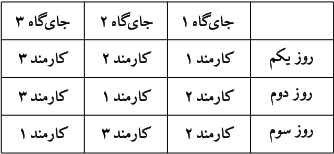
\includegraphics{21.png}

	حال ثابت کنید جایگاه و چینش ماشین‌ها در هر دو روز با فاصله ی 
	$n(n-1)$
	یکسان خواهد بود.

	\SOLUTION{
		\p

	}
\end{PROBLEM}